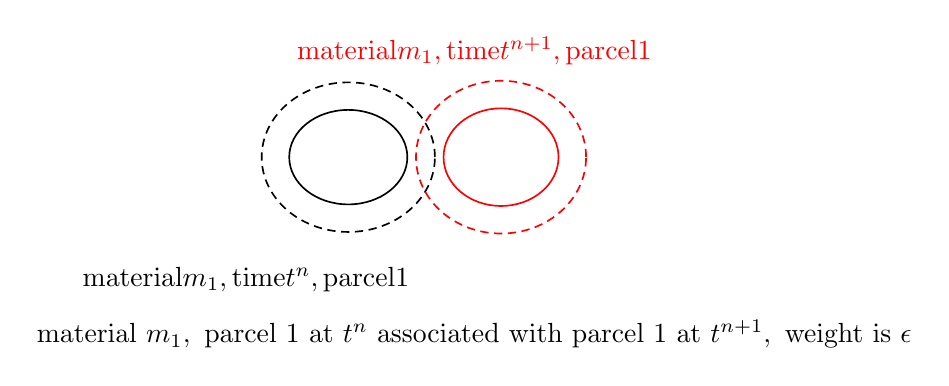
\begin{tikzpicture}

  \draw[semithick] (1,1.95) ellipse [x radius=0.75cm, y radius=0.6cm];
  \draw[semithick, densely dashed] (1,1.95) ellipse [x radius=1.10cm, y radius=0.95cm];


  \draw[semithick, red] (2.94,1.95) ellipse [x radius=0.73cm, y radius=0.62cm];
  \draw[semithick, red, densely dashed] (2.94,1.95) ellipse [x radius=1.08cm, y radius=0.97cm];

\node at (-0.3,0.4) {$\mbox{material}\text{ }m_1,\mbox{time}\text{ }t^{n},\mbox{parcel}\text{  }1$};

 \node at (2.6,3.3) {$\textcolor{red}{\mbox{material}}\textcolor{red}{\text{ }}\textcolor{red}{m_1,\mbox{time}}\textcolor{red}{\text{ }}\textcolor{red}{t^{n+1},\mbox{parcel}}\textcolor{red}{\text{ }}\textcolor{red}{1}$};



\node at (2.6,-0.3){$\textcolor{black}{ \mbox{material } m_{1},\mbox{ parcel } 1 \mbox{ at } t^{n} \mbox{ associated with parcel } 1 \mbox{ at } t^{n+1},\mbox{ weight is } \epsilon}$};


\end{tikzpicture}